\documentclass[11pt,a4paper]{article}
\usepackage[utf8]{inputenc}
\usepackage[T1]{fontenc}
\usepackage{amsfonts}
\usepackage[french]{babel}
\frenchbsetup{StandardLists=true} % à inclure si on utilise \usepackage[francais]{babel}
\usepackage{enumitem}
\usepackage{amssymb}
\usepackage{amsmath}
\usepackage[left=2cm,right=2cm,top=2cm,bottom=2cm]{geometry}
\usepackage{multirow}
\usepackage[dvipsnames]{xcolor}

\usepackage[T1]{fontenc}
\usepackage{fouriernc}
\usepackage{graphicx}

\usepackage{setspace}
\singlespacing

\usepackage{pstricks}
\usepackage{xkeyval}
\usepackage{pst-labo}


\usepackage{multicol}
\usepackage{caption}
\usepackage{fancyhdr}
\pagestyle{fancy}
\renewcommand\headrulewidth{1pt}
\fancyhead[L]{Lycée Denis Diderot }
\fancyhead[R]{Classe de Terminale}
\setcounter{page}{4}\fancyfoot[C]{page \thepage}
\fancyfoot[R]{Année 2025 2026}
\fancyfoot[L]{Alexis RUIZ}
\usepackage{multirow,tabularx,booktabs}
\newcommand{\cadreblanc}[1]{%
\medskip\framebox[\linewidth][c]{%
\rule{0mm}{#1mm}}\par
\medskip}

\usepackage{awesomebox}
\setlength{\aweboxvskip}{0mm}
\usepackage{pifont}
\usepackage{chemmacros}
\chemsetup{modules=all}

\renewcommand{\arraystretch}{2}
\newcommand*\acocher{\quitvmode{\fboxsep0pt \fboxrule0.8pt \fbox{\vrule height1.8ex depth.1ex width0pt \vrule height0pt depth0pt width1.9ex }}}

\newcommand{\defproblem}{\awesomebox[black]{2pt}{\rotatebox{90}{\large{\textbf{Problématique}}}}{black}}
\newcommand{\defconclusion}{\awesomebox[black]{2pt}{\rotatebox{90}{\Large{\textbf{Conclusion}}}}{black}}
\newcommand{\defbox}{\awesomebox[black]{2pt}{
\includegraphics[scale=0.5]{images/appel exam.png}}{black}}


\frenchbsetup{StandardLists=true}
\begin{document}



\center \LARGE{TP2 - Autres réactions d'oxydo réduction}
\\[0,3cm]

\normalsize

\hrule\
\\[0,2cm]

\flushleft \textbf{NOM :\\
Prénom:\\[0,2cm]
}
\hrule\
\\[0,2cm]

\textbf{Expérience 1 :} Dans un tube à essais verser quelques millilitres de solution de sulfate de fer et introduire une tournure de cuivre. \\[3mm]

\defbox{\fbox{
\begin{minipage}{14cm}{
\textbf{Noter vos observations : }\\
\vspace{1cm}
}

\end{minipage}
}}
\vspace{5mm}
\hrule\
\\[0,2cm]

\textbf{Expérience 2 :} 

\ding{202} Dans un tube à essais verser quelques millilitres de solution de nitrate d'argent et introduire une tournure de cuivre.\\
Après avoir attendu quelques instants, représenter sur le schéma ci-dessous le résultat de votre expérience puis noter vos observations :  

\begin{center}
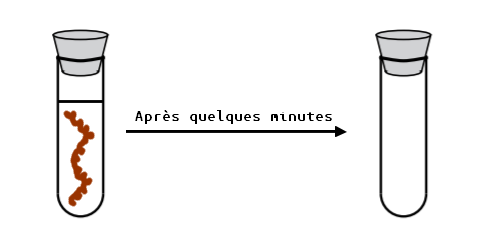
\includegraphics[scale=0.5]{images/tube a essais.png} 
\end{center}

\defbox{\fbox{
\begin{minipage}{14cm}{
\textbf{Observations}\\
\vspace{1.5cm}
}

\end{minipage}
}}
\vspace{5mm}

\ding{203} Filtrer la solution à l'aide d'un entonnoir muni d'un papier filtre puis verser 3 gouttes de soude. 

\begin{center}
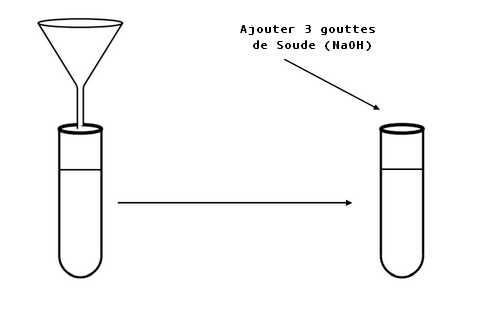
\includegraphics[scale=0.5]{images/filtation entonnoir.png} 
\end{center}



\defbox{\fbox{
\begin{minipage}{14cm}{
\textbf{Observations}\\
\vspace{1.5cm}
}

\end{minipage}
}}

\ding{204}\textbf{ Interprétations : }
\begin{center}

\fbox{Les ions \ch{Ag\pch[]} sont réduits à l'état métallique  : $~~..... ~~+ ~~.....~~ \longrightarrow~~..... $}\\

\vspace{5mm}

\fbox{Le cuivre métallique  \ch{Cu} est oxydé et  donne naissance à des ions \ch{Cu\pch[2]}  : $~~..... ~~\longrightarrow~~.....+ ~~.....~~  $}
\end{center}

On peut aussi dire : 
\begin{itemize}
\item Les ions \ch{Ag\pch[]} ont \textbf{oxydé} le cuivre : l'ion \ch{Ag\pch[]} est un \textbf{oxydant}.
\item Les ions \ch{Ag\pch[]} ont été réduits par le cuivre, le cuivre est un \textbf{réducteur}. 
\end{itemize}

\ding{205} Écrire l'équation globale de la réaction : \\[3mm]

$$~~....... ~~+ ~~.......~~ \longrightarrow~~.......~~+ ~~....... $$

\textbf{\ding{206} Rangement du poste de travail : }
\begin{itemize}
\item Récupérer le contenu des tubes à essais dans le bêcher identifié "Récupération des produits usagés" .
\item Laver la verrerie à l'eau.
\item Ranger la verrerie, le matériel utilisé sur le chariot. 
\end{itemize}



\end{document}